% Install the VS Code extension to view the PDF rendering in a tab
\documentclass{report}
\usepackage{fullpage}
\usepackage[T1]{fontenc}
\usepackage[mathletters]{ucs}
\usepackage[utf8x]{inputenc}
\setlength{\parskip}{.8em} 
\usepackage{graphicx}
\usepackage{listings}
\usepackage{color}

\definecolor{dkgreen}{rgb}{0,0.6,0}
\definecolor{gray}{rgb}{0.5,0.5,0.5}
\definecolor{mauve}{rgb}{0.58,0,0.82}
\graphicspath{ {./scatters/} }

\lstset{frame=tb,
	language=Java,
	aboveskip=3mm,
	belowskip=3mm,
	showstringspaces=false,
	columns=flexible,
	basicstyle={\small\ttfamily},
	numbers=none,
	numberstyle=\tiny\color{gray},
	keywordstyle=\color{blue},
	commentstyle=\color{dkgreen},
	stringstyle=\color{mauve},
	breaklines=true,
	breakatwhitespace=true,
	tabsize=3
}


\begin{document}
	\begin{flushleft}
		\huge CS 415 Project 1
		
		\normalsize Keegan Donley, Jeff Hultman

		\section{Task 1}

		\paragraph{Average-case efficiency of Euclid's algorithm and consecutive integer checking algorithm}
		To test the average-case efficiency of these algorithms, we generate
		100 values of n from 1 to 70, then count the number of
		operations needed to calulate the average GCD for n using
		Euclid's algorithm and consecutive integer checking.

		To calculate the average number of operations for n, we take the average
		number of operations for:
		
		euclidGCD(n, 1), euclidGCD(n, 2), . . . , euclidGCD(n, n)

		and

		consecutiveGCD(n, 1), consecutiveGCD(n, 2), . . . , consecutiveGCD(n, n)

		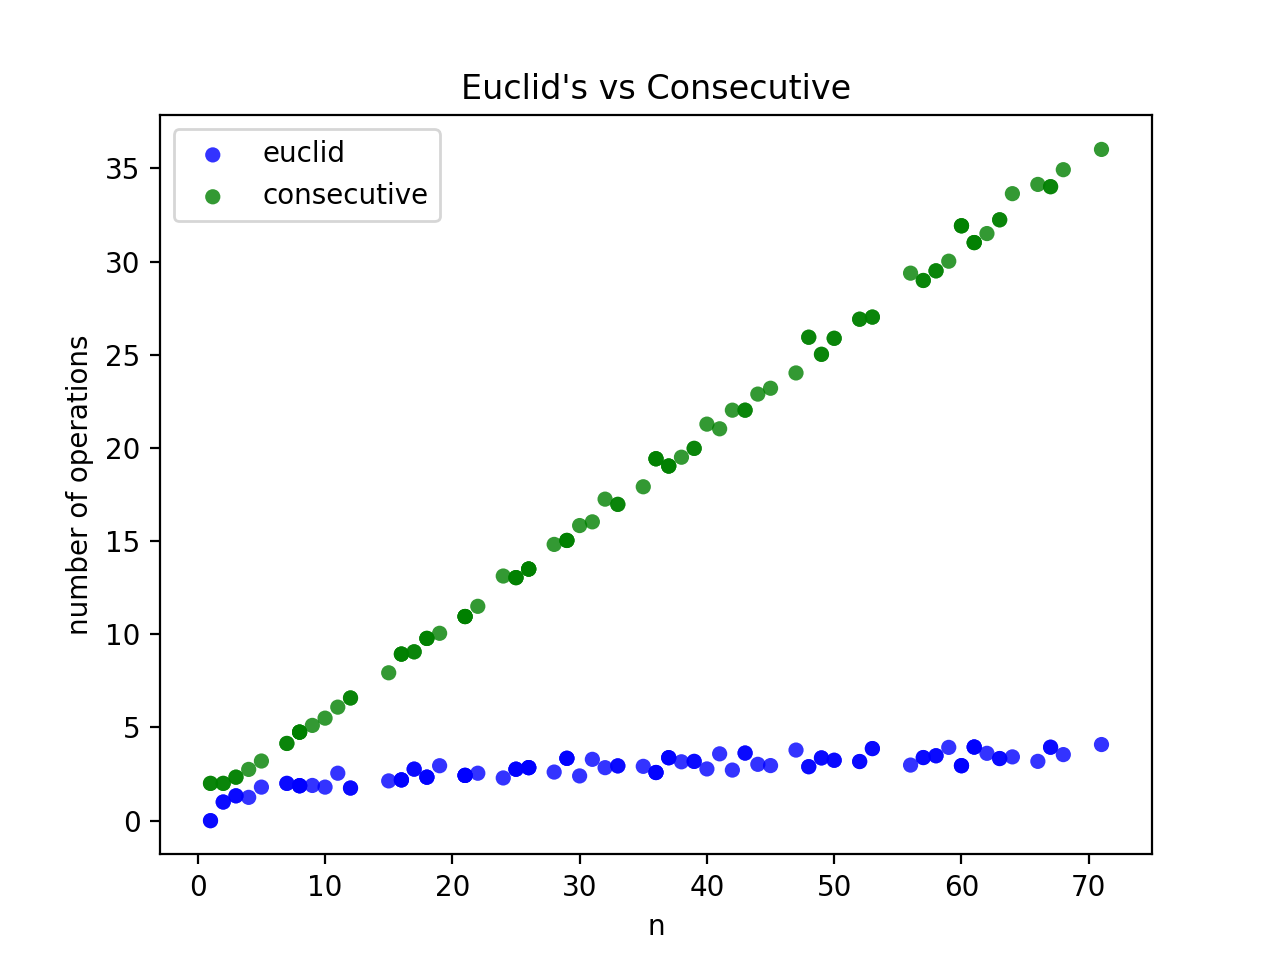
\includegraphics{task1}

		\textbf{Euclid} $\theta$(logn)

		In the average case, Euclid's algorithm runs in $\theta$(logn) time and took less than 
		5 modulo divisions.
		
		\textbf{Consecutive Integer} $\theta$(n)

		The empirical testing shows the consecutive integer testing results to be nearly perfectly linear.

		\section{Task 2}

		\paragraph{Worst-case efficiency of Euclid's algorithm}
		The worst case for Euclid's algorithm occurs when two consecutive integers from the Fibonacci sequence are used as m and n. To test
		the efficiency, we generate 200 values for k between 1 and 200. k is an index in the Fibonacci sequence, where m = k + 1 and n = k.

		For example, based on the start of the Fibonacci sequence: [0, 1, 1, 2, 3, 5, 8, 13, 21, 34, 55]

		k = 5 => gcd(8, 5)

		k = 8 => gcd(34, 21)

		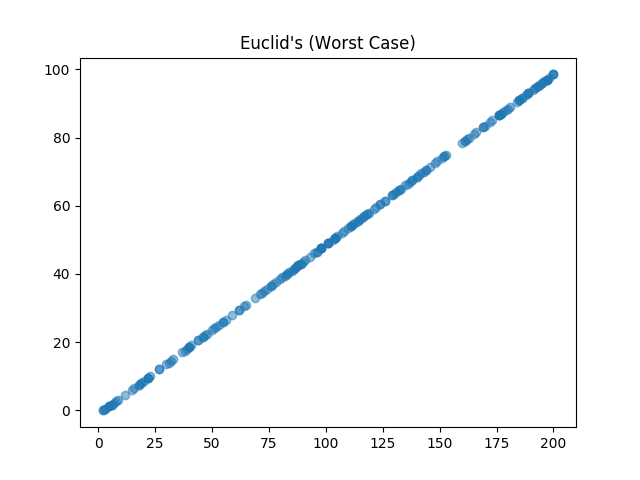
\includegraphics{task2}

		Because the gcd of two consecutive Fibonacci numbers is always 1, the complexity in the worst case for Euclid's algorithm
		is $\theta$(logn). We saw a trend that respresents a complexity of $\theta$(logn) in the average case as well, however the number
		of modulo divisions tended to be lower than how many were needed in the worst case.

		\section{Task 3}

		\paragraph{The "middle-school procedure"}
		To evaluate the complexity of the middle school method of calculating GCD, we generated 1000 pairs of integers from 1 - 999 as m and n. When plotted, the results
		show that the middle school method is $\theta$(n).

		On the x axis, we plotted max(|prime factors in m|, |prime factors in n|) against the y axis - the number of operations needed
		to compute the GCD. The basic operation is the comparison of prime numbers.

		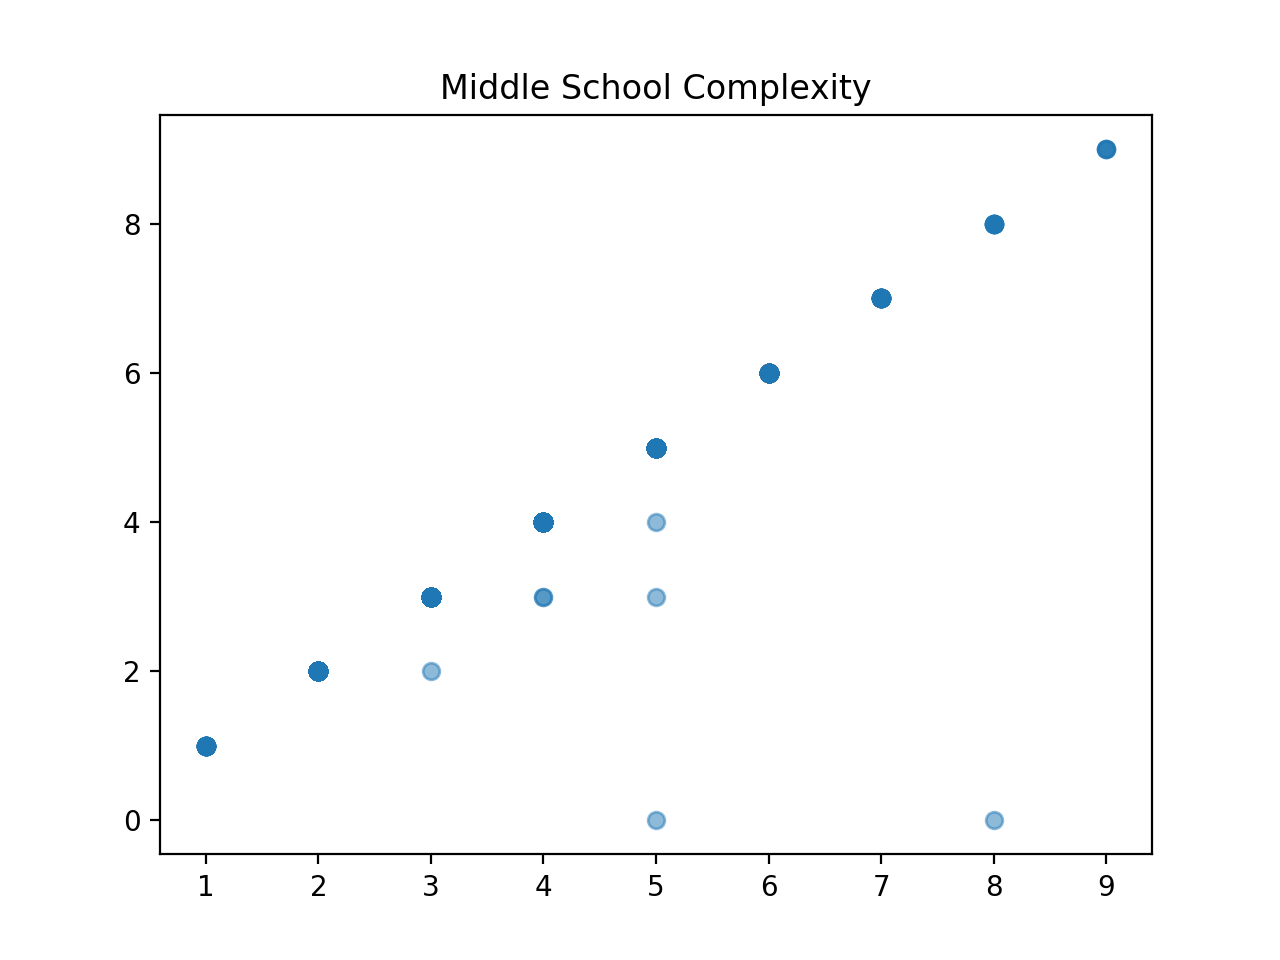
\includegraphics{task3}

		The evidence shows the complexity to be approximately linear, but there are some outliers where 
		both m and n had prime factors, but none were common and the gcd was determined to be 1.


	\end{flushleft}
\end{document}